%!TEX root = thesis.tex

\chapter{Introduction}
\label{chap:intro}

The success of the technological advances often can be associated with an unprecedented convenience that they bring in. At the heart of this convenience lies the ability to relax the limitations of the human body to a certain extent. From this point of view, it is not a surprise that the three most prominent technological wonders of the last century, namely the \emph{Television}, the \emph{Telephone} and the \emph{radio} (which was originally called \enquote{radiotelegraphy}), bears the same Greek prefix \emph{tele-} which corresponds to \enquote{\emph{at a distance}} in our context. This shows that there is something of extreme importance about our drive to extend our capabilities beyond the constraints that our bodies impose.


It is quite remarkable, in retrospect, that these \enquote{gadgets} did not perish but rather kept on evolving since initially they were far from perfect. Quite the contrary, they were hardly operational. Even the commercialized version of the early TVs had a narrow bandwidth and minimum image quality. Similarly radio and telephone was barely transmitting sensible information as far as the signal-to-noise ratio is concerned. Nevertheless, they have provided the ways of communication which were unimaginable before their time. Therefore the added value dominated the shortcomings and even though they were quite imperfect, we kept using them. The important lesson to be learned is that a technology should not be judged by its imperfections but rather should be weighed by its contribution in this context and the convenience that is either immediately brought in by using it or its foreseen potential by the \enquote{early adopters}.

The success is also related to the fact that these technologies mainly relied on the human brain itself at their early stages. For example, the human brain did most of the noise filtering and data recovery by just guessing the missing pieces and identifying patterns from the signal brought by the respective medium. Today, with our smart mobile phones and 3D LED TVs, we can assume that the computational load on the human brain is drastically reduced. In other words, it's true that we are still identifying patterns and utilizing the relevant parts of our brain to make sense of a TV broadcast\footnote{Pun intended.}. However, we don't need to use a higher level of concentration to reconstruct the words that we hear or to identify the image on the display thanks to the high quality output. We can not exaggerate the importance of the human brain and its immersion power. 

Leaving essentially the same footprints, we are on the same track with the technological developments involving our touch sense. Though various science fiction items already used such ideas extensively, the real technology tends to follow from quite a distance.  Considering the importance of our touch sense in any given situation, the added value of extending of our perception in this modality needs no motivation. Take the most familiar, the vibrating mobile phone in the silent mode in our pocket. This is a very important example since every individual learns what that vibration might mean, either an SMS or a call, depending on the vibrational pattern. This means that the touch sense can be used to convey messages and more importantly we can process those messages for inference which forms the basis of the so-called \enquote{haptics} and haptic technology.


The type of information from the cell-phone example is said to be received via the haptic channel (or the collaborative use of tactile and proprioceptive modalities). At this point we have to emphasize that, we use the term \enquote{touch sense} pretty vaguely as a shortcut and we leave it to the experts of the field to define the sophisticated mechanisms (pertaining to the somatosensory system) that we utilize when we manipulate objects, say with our bare hands. 


Since our skin and muscles form one of most sophisticated and complex sensory systems, the somatosensory system, the brain can easily interpret the slightest changes and this extra signal processing power gives us a chance to hack into this system by providing artificial inputs via haptic displays. Still, it is rather conspicuous that this is impossible to achieve a total immersion with today's technology. The essential complication is twofold: the high sensitivity of the very same sensory system makes it difficult to fake or mimic a natural phenomenon by artificial means and on the other hand we do not have a well-defined mapping from the to-be-created sensation to the required excitation signals. Moreover, even if we have such mappings available, the related hardware must execute the computed haptic signal profiles perfectly which is generally not the case.

Then, we could simply ask \emph{Why bother?} 


\section{The Objectives}
\label{sec:intro:obj}

We first give a summary about the current concepts of the involved technology (as we foresee from a narrow \enquote{today's} perspective) and later on, define our microscopic focus of this thesis in this vast generality. This would hopefully provide additional insights to what follows in the later sections.  


The touch related applications are diverse. The diversity is not only in terms of sensation they are related to (texture, shape etc.) but also how they encode the information and transmit via various modalities (e.g. vibrational patterns in mobile electronics, variable resistance to motion in game consoles and steering wheels etc.). There is no particular reason to limit ourselves with the daily needs or even luxurious demands regarding our touch sense as mobile phones taught us that a vibration in our pocket means a contact request from someone which is hardly ever related to the touch sense. This should be pretty awkward to experience if someone actually would come and shake our pockets to draw our attention (unless it is socially accepted). Therefore, we have devised a way to translate one particular message into another by simply teaching ourselves and getting used to it. Thus, it does not seem improbable that other types of physical units in terms temperature, light intensity etc. being converted into pressure or tactile patterns in time domain.

Hence, it is our belief that the crux of this technology is establishing a interpretable protocol between our brain and the machine but not exactly reflecting the particular state of some distant or virtual physical medium. 
This would be the main argument of this thesis when we distinguish our approach with its comparable counterparts. For this reason, we would like to narrow down our focus further by defining different types of touch related concepts.

\subsection{A Terminological Classification}

As we mentioned above, the somatosensory system is quite complex and there are different layers of sensory mechanisms that contribute to the overall perception. The main two branches of technology relating to the touch perception are the tactile and kinesthetic  feedback. The terminology is yet to reach a steady-state standard however what follows below is plausible considering the variations and nuances found in the literature. Since there is no fixed definition for such perception we would use a rough  classification based on the amplitude-frequency of the motion. We have to emphasize that this classification is completely conceptual and only serves to exclude the parts that are not studied in this thesis. Therefore, we refer the reader to the authoritative resources of the involved physiology, e.g., \cite{kandel}. We start with a somewhat detailed sensory classification to support our choice of amplitude-frequency based grouping.

Typically, the touch perception is classified into two groups. Tactile feedback and kinesthetic (proprioceptive) feedback. For practical purposes, one can use the analogy of a parallel connected high-pass and low-pass filter. For our control-oriented context, let us define a few key concepts with an engineering point of view. 

In physiology, the sensors on the skin which take different physical measurements, are called \emph{receptors} and prefixed with their area of specialization such as \emph{thermoreceptors, mechanoreceptors, nocioreceptors}(pain) etc. The signals that trigger an action on these receptors are denoted as the \emph{stimuli}. In case of a stimulus, these receptors, through some chemical processes, exhibit a series of \emph{action potentials} or electrical discharge pulses i.e. a \emph{spike train}. In the engineering terminology, this can be modeled as a nonuniform Dirac comb with varying frequency as a function of the stimuli intensity or a digital frequency modulation (FM) signal. The frequency increases with the stimulus intensity. Furthermore, at the input side of this sensor there is a dead-zone nonlinearity hence the stimuli should exceed a particular threshold to trigger a receptor firing.

There is also another process, \emph{neural} or \emph{sensorial adaptation} which quantifies the frequency decay of firing under constant stimulus. We can see the tangible effect of this process frequently e.g., our nose looses the sensitivity to a powerful smell if exposed to it for some time or we stop noticing the touch of the glasses on the face or the ring on the finger. Some sensors have a slow decay rate whereas others decay in a matter of seconds. The slow sensors often called the \emph{slowly adapting(SA)} and others are called \emph{fast adapting (FA)} or \emph{rapidly adapting} type \cite{burdea}.


As shown in \Cref{tab:mechano}, and also surveyed in \cite{kontarinis}, there are four main types of mechanisms that are utilized for the force and texture sensing with varying operating conditions and spatial authority. Although all contribute to the high frequency stimulus perception with varying levels, slowly adapting receptors are mainly tuned to detect the low frequency information range (up to \SI{30}{\hertz}). The fast adapting Meissner(FAI) and Pacinian(FAII) Corpuscles can be excited in the frequency range of \SIrange{10}{60}{\hertz} and $\SIrange{60}{1000}{\hertz}$ respectively. Thus, small-area receptors (Type I) are excited with rate of skin deformation whereas relatively large-area receptors (Type II) are with the acceleration of the skin. Moreover, FAI units are located closer to the skin surface, have high unit density with small surface area forming a grid of sensors. On the other hand, FAII units are located in the subcutaneous tissue and work as a single load cell with relatively large surface area. This allows experts to assume that FAI units are mainly responsible for spatial information about the skin deformation and FAII units are responsible for the high frequency information with response delays in the range of \SIrange{50}{500}{\milli\second} \cite{idareview}. Another interesting note in \cite{kontarinis} is that due to their single unit nature FAII units offers the possibility to provide high frequency information with a single vibration display but for FAI units it is more appropriate to supply an array of haptic displays for lower frequency range.  

The SAI disk receptor has a small, localized receptive surface area as opposed to the SAII with a large field with a decaying sensitivity from center to the edges. Individual Ruffini endings are excited by stretch of the skin in specific directions. The majority of hand receptors consists of FAI units ($>40\%$), then SAI units are almost a quarter which followed by SAII covering $19\%$ and FAII $13\%$. 



\newcolumntype{C}{>{\centering\arraybackslash}m{1.9cm}}%
\begin{table}%
\centering
\caption[Functional Features of Cutanous Mechanoreceptors]{Functional Features of Cutanous Mechanoreceptors (Adapted from \cite{idareview})}
{\tiny
\pgfplotstabletypeset[
column type=C,
every head row/.style={before row={\toprule},after row=\midrule,},
every last row/.style={after row=\bottomrule},
every even row/.style={before row={\rowcolor[gray]{0.9}}},
col sep=&,row sep=\\,
string type,
]{
Feature	                   &Meissner Corpuscles (FAI) &Pacinian Corpuscles (FAII) &Merkel's Disks (SAI) &Ruffini Endings (SAII)\\
Rate of adaptation         &Rapid                     &Rapid                      &Slow                 &Slow\\
Location                   &Superficial dermis        &Dermis and subcutaneous &Basal epidermis &Dermis and subcutaneous\\
Mean receptive area        &\SI{13}{\milli\metre\squared} &\SI{101}{\milli\metre\squared} &\SI{11}{\milli\metre\squared} &\SI{59}{\milli\metre\squared}\\
Spatial resolution         &Poor&Very poor&Good&Fair\\
Sensory units              &43\%&13\%&25\%&19\%\\
Response frequency range   &\SIrange{10}{200}{\hertz}&\SIrange{70}{1000}{\hertz} &\SIrange{0.4}{100}{\hertz} &\SIrange{0.4}{100}{\hertz} \\
Min. threshold frequency   &\SI{40}{\hertz}&\SIrange{200}{250}{\hertz} &\SI{50}{\hertz}&\SI{50}{\hertz}\\
Sensitive to temperature   &No&Yes&Yes&At $>\SI{100}{\hertz}$\\
Spatial summation          &Yes&No&No&Unknown\\
Temporal summation         &Yes&No&No&Yes\\
Physical parameter sensed  &Skin curvature, velocity, local shape,flutter, slip &Vibration, slip, acceleration &Skin curvature, local shape, pressure&Skin stretch, local force\\
}
}% Closes the \tiny group
\label{tab:mechano}
\end{table}

\subsubsection{Weber ratio and Just-Noticeable-Difference(JND) }

Weber ratio is defined as the ratio between the minimal stimulus intensity change in any physical quantity that triggers a change perception and the intensity of the stimulus. In case of a constant or static stimulus the ratio is denoted with Just-Noticable-Difference (JND). For engineering purposes this derived unit can be beneficial to design the frequency behavior of the haptic systems which exhibit a particular sensitivity pattern.


\subsubsection{Tactile Feedback}

Tactile feedback, in general, is utilized to distinguish fine details such as shape, curvature, vibration, acceleration, and texture perception. Hence, the high-frequency content of the touch information is indispensable to transmit such information. Since the amplitude of the motion at these frequencies are quite small, the palm and finger tissues act as a low-pass filter and avoid such information to penetrate into the skin. Thus, only a limited part of the sensors have access to this information.

A striking example to the mind-boggling quality of feedback is the Braille system used by visually impaired or disabled individuals (\Cref{fig:braille}). The average reading speed with Braille system is about 125-150 words per minute (\cite{americanblind}) in contrast with 200-250 words per minute by eyesight. 

\begin{figure}%
\centering
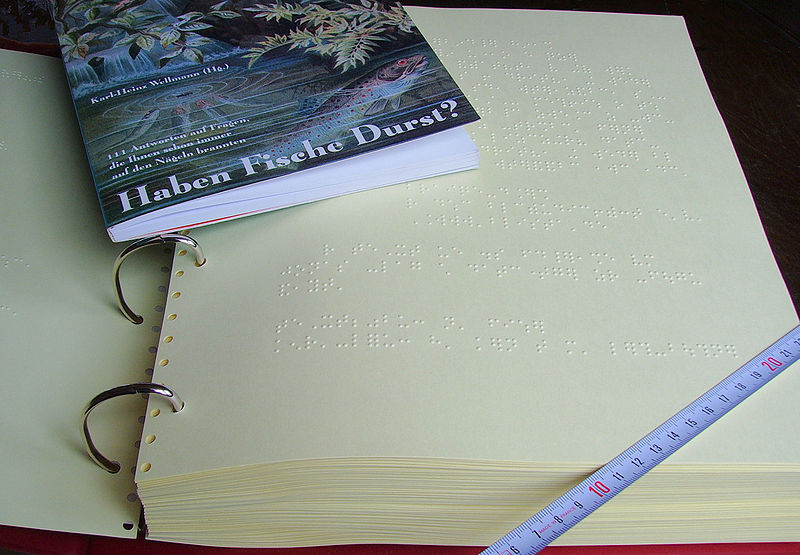
\includegraphics[width=0.8\columnwidth]{\impath/intro/braille.jpg}%
\caption[The length comparison of the same content in the form of Braille and 
regular text]{The length comparison of the same content in the form of Braille and 
regular text (Source: Karl-Heinz Wellmann, 
\href{http://de.wikipedia.org/wiki/Brailleschrift}{[Wikipedia:Brailleschrift]})}%
\label{fig:braille}%
\end{figure}

Most of today's technological devices utilize this modality to send and receive information. Many mobile phone applications and a few gaming consoles such as Nintendo Wii\raisebox{0.5ex}{\scriptsize\texttrademark}, Sony Playstation\raisebox{0.5ex}{\scriptsize\texttrademark} etc., utilize short vibrational patterns to alert the user that some action has been performed e.g. the user hovers over a hot spot on the screen or some moving object hits an obstacle etc. 

The tactile technology is, thus, concerned with the vibrational pattern and high-frequency sweep of stimuli. Communication via small vibrational or textural subtleties allows the tactile technology to focus on the low-stroke, high-bandwidth haptic displays. The required low-stroke action is often generated by a small and agile electrical motor with a load eccentricity with respect to the rotor shaft axis. The angular velocity of the motor then defines the frequency of the vibration. Since the involved mechanisms on the human limbs and hands are rapidly adapting, the bus speed in this modality can be very high compared to the kinesthetic feedback in which the human should track and pick out patterns from relatively slow and large-amplitude motion profiles via measuring muscle stretch amount and various other quantities. 


\subsubsection{Kinesthetic (Proprioceptive) Feedback}
Proprioception\footnote{We will not go into the nuances between kinesthetic and proprioceptive feedback} (\emph{Proprius}+\emph{perceptio}: the act of gathering of own) is the ability to sense the body position and motion without using the visual aid. Kinesthetic feedback, together with limited force sensing abilities of muscles and tendons and relatively small interference of tactile feedback system, is \enquote{vital} to have control of our own body. It's a futile attempt to describe the importance of this often overlooked perception (or hidden sense) other than referring to the shocking 1998 BBC \emph{Horizon} documentary \enquote{\emph{The man who lost his body}} and the paper \cite{waterman} about Ian Waterman. He is the only person known to date who can cope with the loss of proprioceptive feedback while still being able to stand up, walk, maintain posture etc. without any artificial support. Unfortunately, he is completely dependent on his visual feedback as he tirelessly computes trajectories of his body parts on-the-fly to compensate for the loss of kinesthetic feedback even when gesturing with hands. 

Thus, whether we are aware of it or not, proprioception is indispensable for us to survey the environment. The force on our limbs, our body configuration at that instance, and body motion are sensed via sensors in the joints, muscle tendons and muscles themselves. Unlike the tactile feedback characteristics given previously, the compliance, the distribution of pressure and and the shape information is measured in a relatively coarse fashion. Hence, when combined with tactile feedback and the brain's internal comparison database we use an unparalleled sophistication to actually perceive the environment without using any visual feedback even the object is foreign to us. In \cite{biggssrinivasan}, a convenient summary of the properties is presented. Distilling even further for a general picture about the proprioception, we provide the following quick facts. 

The compression or stretch of the receptors covered previously changes the amplitude of the impulse of the action potential which in turn used as the position information. Similarly the frequency of these firings are interpreted as the velocity information. For the limb position and motion, the bandwidth of the kinesthetic sensing is around \SIrange{20}{30}{\hertz} with varying accuracy in terms of JND around \SIrange{0.8}{2.5}{\degree}. Moreover, the control bandwidth is reported to be task-dependent: \SIrange{1}{2}{\hertz} for unexpected signals; \SIrange{2}{5}{\hertz} for periodic signals, \SI[parse-numbers=false]{<5}{\hertz} for generated or learned trajectories and finally about \SI{10}{\hertz} for reflex actions. 

Regarding the force sensing, it has been experimentally demostrated that pressure JND decreases as the pressure area increases e.g., overall average JND drops to $3.7\%$ with a contact area of \SI{20.27}{\centi\meter\squared} from $15.6\%$ with a contact area of \SI{1.27}{\centi\meter\squared}. 

The kinesthetic technology can be used in conjunction with tactile technology to provide a full manipulative immersion. Moreover, in the case of \emph{exoskeletons}, it can be the essential ingredient to protocol between the environment and the human body. Especially, rehabilitation patients can benefit from such technologies via combining the visual and the kinesthetic feedback to amplify the disabled or impaired control action of the problematic limb. Thus, kinesthetic technology is mainly involved as low-frequency based manipulative or explorative motion tasks. Considering the current hardware limitations, many tasks depend primarily and rather primitively kinesthetic cues for bilateral teleoperation and virtual reality applications.


\subsubsection{Teleoperation}
Teleoperation is the general name for providing human actions to a different media that is not accessible (or only in a costly way) to direct contact in a precise fashion. Microcomponent assembly, minimal invasive surgery (MIS), space station maintenance and construction, underwater exploration and construction are all typical application examples that the human either can not be present or physically interact with comfortably. The \emph{da Vinci}\raisebox{0.5ex}{\scriptsize\texttrademark} surgery robot from Intuitive Surgical Inc. is a well-known example of \emph{unilateral} human manipulation to achieve high precision tracking with surgical tools inside very tight incision (with other qualities that are not relevant to enumerate here). 

However, as often motivated by the \emph{bilateral} teleoperation studies, the human operators, expecially the experienced ones, often lack the ability to employ their precise tactile and kinesthetic abilities to take decisions or to monitor their progress since they rely on vision feedback from the cameras exclusively. In some particular practices, surgeons might resort to inserting their fingers inside the incision to feel the relevant tissue stiffness difference to get a better spatial understanding when the view is contaminated with blood or other bodily fluids. In the case of an obstruction during an insertion of an instrument into the body, they might tend to correct the instrument based on their force feel at hand. Hence, the realism is diminished as opposed to the increased precision by the teleoperation methods. 

\subsubsection{Bilateral Teleoperation}

Bilateral teleoperation is simply teleoperation equipped with force feedback to the human operator with the hope to increase the realism by recreating the force vectors of the distant medium at the local environment. The majority of the bilateral teleoperation research is on the kinesthetic feedback. In particular, the human interacts with the local device by moving a constrained handle to explore the environment or using a stylus-like stick. Hence, the experience is mostly based on the success of imitating a physical tool. Therefore, the tactile cues are of secondary nature. The challenge of course is to increase the performance level to a tactile display level while still maintaining the tool usage capability. The particular MIS tasks that are performed with a scalpel are one of the hot topics of todays research effort and it requires not only kinesthetic feedback, though a major accomplishment by itself, but tactile feedback too, for understanding the nature of the texture or the stiffness of the tissue. Similarly teleoperated peg-in-hole type of tasks are also a major area of investigation e.g., ground-satellite robotic mission directives or underwater construction tasks would benefit much from such possibilities to reduce the operational cost, duration, and success rate. 



There are many interesting challenges when it comes to this recreation process. For example, in a microassembly task, the experienced forces are substantially different than what we feel during daily tasks. Gravity is our main source of reference when interpreting a distant location, however, gravity becomes almost negligible in the micro domain as adhesive forces such as Van der Waals, electrostatic and surface tension forces dominate (the most common example is that the parts that are picked up in microdomain tend to stick to the tweezers). 

If we manage to create a believable level force feedback sensation in these otherwise inaccessible domains, there are a few very important quasi-philosophical and also task-dependent questions that need to be answered. A few of these questions are:

\begin{itemize}
	\item Should the device reflect those forces to the human operator for the sake of realism which are utterly counter-intuitive and even worse appear to be happening at random? 
    \item Is there any correlation between increased realism and increased comfort? In case of a difficult task, what good the realism bring in by replicating the difficult task at a distant location in the local environment?
    \item Do we need to reflect the human motion to the remote location perfectly since that is a waste of resource? In other words, we neglect the fact that a robot can perform certain tasks much more precisely than a human operator. Is there any downsampling/upsampling protocol to vary the motion precision depending on the receiver?
    \item If we decide to filter the unnecessary force information that are related to mental/muscular fatigue, how should we know what to filter? 
    \item Do we use the full capacity of our \emph{internal data bus} to transfer touch information, or put differently, is there any space left to encode other quantities on top of the touch sense?
    \item Can we assume that all users more or less reach to the same understanding given a kinesthetic cue sequence?
\end{itemize}

These questions are indeed quite interesting and challenging. The reason for enumerating a few of them here is that the scope of this thesis reaches to a point just before we are ready to attack them properly. In other words, we will focus on a framework that would help to set up such teleoperation devices such that experts of these fields can use these devices to answer those items above.

\subsubsection[Haptics]{(Computer) Haptics}
In general, haptics technology encompasses all the items that are covered up to this point, however, it is also often used as a placeholder for the concept of creating artificial or virtual object perception with a force-feedback capable device. Computer haptics also have additional challenges such as rendering deformations in case of a soft object or realistic graphical presentation of object interaction in terms of collisions etc. In other words, not only the forces are important but the consequences of these force interactions need to be handled in a precise fashion. Conversely, computer haptics is free from the hardware limitations or the noisy measurements as the objects and the physical laws that they should obey are computer generated. 

\subsubsection{Virtual Reality}

This term refers to a set of artificially generated immersion techniques that can rely on either a single or multiple modalities at once. The common applications consist of special googles that cover the human vision. By tracking the head movements and adjusting the scene that is projected to the special headset, the user can immerse into the artificial environment. Combined with headphones and if possible with haptics, the experience can be substantially improved. Especially haptics can increase the immersion level much more compared to only visual+audio supplements since otherwise the realism can be destroyed quickly if the user tries to touch any object or surface while actually waving his hand. The persuasiveness of the scene depicted on the headset needs to be backed up with at least a slight kinesthetic feedback, if not tactile, since the loss of tactile feedback can be swept under various scenario e.g., the user can be placed in a situation with using blunt items, thick gloves, robotic hands etc. 



\subsection{Structure and Objectives of This Thesis}
Let us turn to our initial question \emph{Why Bother?}. We do because there is no need to obtain the ultimate perfect touch sensation for the human in order to interpret the signals correctly. It is the same principle with LED-TVs. Nowhere on the screen, a color different than Red, Green, and Blue is emitted. However, we tend to approximate the output to the closest color since the emitters are close enough and we achieve the color perception. Therefore, realism is not our primary objective. However, before we even enter this discussion, the teleoperation devices must be stable and should exhibit consistent performance such that experts from neuroscience, psychophysiology, and other related scientific fields can join and assess different ways of protocoling with the human brain in this modality. Otherwise their conclusions would be contaminated by the device properties (we can even speculate that this is often the case, though no proof will be presented here). Thus it is the point of this thesis at which we consider the stability properties and control problem of bilateral teleoperation and we believe that we have achieved a limited success toward this direction.


To restrict the scope of this thesis further, we exclusively stay in bilateral teleoperation concept as we have defined previously and focus on the control theoretical aspects of the teleoperation for a stable interaction with sufficient performance levels. The reason of such a terminological enumeration above is to precisely draw the boundary of what will follow in the later chapters. 

We first give an opinionated version of the literature to point out to the underlying connections between seemingly different methodologies and also provide a simpler explanation to the well-known \emph{wave variables} formalism. By doing so, we classify such methods in the respective mainstream control theory methods and clearly demonstrate that they are indeed outdated if compared to the recent advances. Moreover, we argue that now-standard assumption of \emph{passivity} property on the human and environment is not an experimentally validated one. We also claim that the success of passivity-based methods are due to the conservatism of these tests and not due to the validity of the assumption.

In \Cref{chap:analysis}, we then show also both theoretically and numerically that the frequency methods found in the literature can be combined under one framework via \emph{Integral Quadratic Constraints}. With these results, we demonstrate that the proposed framework of this thesis does not bring in additional complications or conservatism. In fact, via numerical case studies, we show that the results are precisely the same. Therefore, there is no fundamental reason to use a specialized terminology of the networks and microwave systems which in turn alienates mainstream control theory experts. We also remark that uncertainty modeling is a key aspect in obtaining better controllers for bilateral teleoperation. To highlight the reasons why we promote this framework, we also give examples of different combinations of uncertainties for which classical tools that are employed in the teleoperation literature are not suitable but already available in the robust control literature for already 15 years. 


After establishing this link with the methods in the literature we turn to the controller synthesis problem in \Cref{chap:synth}. We formulate the problem as a generalized plant and work out scarce details that are found in the literature to obtain a better model-based control synthesis algorithm using static and dynamic IQCs. We also explicitly identify what the bottlenecks are for the interested reader.  

In \Cref{chap:conc}, we provide some concluding remarks and for the reader's convenience, in \Cref{chap:apdxnetwork}, we recap the basics of the network theory.

